\section{The price of the search}
\label{sec:price-search}

The postulates of Section~\ref{sec:passive} say that the meter cannot be cheated.
This section says what the meter reads, by grounding each postulate in the
sharpest current results, and it reports one experiment. Everything here carries
its epistemic status inline, because the ground shifts: two of the units this
section could have been built on two years ago are now known to be
algorithm-relative artifacts.

\subsection{The price of aiming}
\label{sec:price-aiming}

The no-aiming postulate says the only search over model space is learning. Its
concrete form is a lower bound on the oracle cost of any generic adversary that
must produce a model with a target property, and the bound depends on the query
type the recipe's steps realize.

For recipes whose steps are statistical queries, the floor is unconditional. A
hidden $k$-sparse parity requires $d^{\Omega(k)}$ statistical queries at any
useful tolerance, and this is the number Barak et al.\ describe SGD as
approaching \cite{BEGKMZ22}. For Gaussian single-index models the current sharp
single number is the generative exponent $k^*$: any statistical-query algorithm
that outputs a direction with nontrivial overlap needs $n \gtrsim d^{k^*/2}$
samples, unconditionally within the class \cite{DPLB24}. One caveat travels with
that citation and it runs in the safe direction: the authors state that their
theorem primarily measures the detection threshold, and the statistical-query
estimation threshold is open, so the true price of recovery can only be higher
than the floor quoted here. For multi-index models the same quantity governs
subspace recovery, with an unconditional estimation upper bound at the matching
rate and a low-degree lower bound \cite{DLB25}. Any reading of the low-degree
half as polynomial-time hardness must carry the refutation of the
quasi-polynomial low-degree conjecture and its surviving positive counterpart
\cite{BHJK25,HKKLMT26}.

Two units this section does not use, and why. The information exponent prices a
single algorithm, online SGD from a random start \cite{AGJ21}, and the leap's
lower bound holds for correlational statistical queries only, with its SGD side
an open conjecture \cite{ABM23}. Both thresholds collapse under batch reuse
\cite{DTAPZK24}, and the collapse is not an anomaly: reuse reaches the
information-theoretic rate for polynomial links \cite{LOSW24}, a learning-rate
schedule induces the same transition without carrying any sample across
iterations, though each sample is queried twice within its own iteration
\cite{TME25}, and full-batch descent separates from one-pass descent, with the
separation proved for a truncated variant of the target and provably absent for
the plain one \cite{KJWSM26}. What survives this wave is the generative exponent, whose
defining invariance is exactly closure under the transformations reuse exploits
\cite{DPLB24}. Proven, all of it, in the classes named.

The structural escape calibrates the postulate rather than refuting it.
Noiseless parity is solvable by Gaussian elimination from $O(d)$ samples, an
algorithm that manipulates samples algebraically and is no statistical-query
algorithm. In the framework's terms that is a structural attack, and parity is
the case where the win-win of Proposition~\ref{prop:winwin} is not hypothetical:
the generic floor is $d^{\Omega(k)}$, the structural attack is linear algebra,
and the gap between them is a named theorem about what learning-shaped
computation cannot do.

\subsection{The price of skipping is recipe-relative}
\label{sec:price-skipping}

The no-skipping postulate as stated in Section~\ref{sec:passive} prices the
walk of one recipe. The literature now forces exactly that scoping, and the
force is worth exhibiting, because a stronger reading of the postulate is false.

The walk's length is a property of the pair recipe and query type, not of the
task. The batch-reuse and learning-rate results above shorten the same walk to
the same target by changing the recipe slightly \cite{DTAPZK24,LOSW24,TME25},
and empirically the compute needed to reach a fixed language-model loss has
halved roughly every eight months across a decade of recipe drift \cite{HBEORGATS24}.
So a task-level no-skipping claim is refuted, and a recipe-level one is the
strongest defensible form. Within a fixed recipe, the compute-to-loss frontier
is a theorem in solvable models: for power-law random features under one-pass
stochastic gradient descent the loss curve is exact and the compute-optimal
frontier is a derived object \cite{PPXP24}, which is the theorem-shaped form of
the empirical scaling laws \cite{KMHBCCGRWA20,HBMBCRCHWCHNMDDGOSERVS22}, whose fitted constants
are themselves contested \cite{BEBY24}. The mechanism literature makes the
exponent explicitly algorithm-dependent: allowing feature learning nearly
doubles the compute exponent on hard tasks \cite{BAP25}, and a good data-pruning
rule changes the law's form outright \cite{SGSGM22}. None of these results claims
a lower bound over all algorithms, and no such bound exists. Open, and it is the
open problem under every compute-pricing claim in this survey.

Two consequences are definitional in the oracle model and consistent with the
empirical record. First, amortization is not skipping. Distillation reaches a
target cheaper only when a stronger teacher already exists, and the teacher's
training was an oracle call somebody paid for \cite{BSWRLW25}. In the model, a
party that builds a derivative model builds it from views of prior traces, so
the cost sits upstream in the ledger. There is no free trace, only amortized traces. Second, the
price of a view is not the price of the trace. Proof-of-learning verification
accepts a lossy view of the trace, and the published forgeries attack that view,
succeeding without paying the walk \cite{FJTYCDCP23}, while exact reproduction
of a trace remains empirically out of reach \cite{SHKBL25}. A sound
proof-of-learning is precisely a view whose price equals the trace's, and
whether one exists is the open problem that literature keeps encountering from
inside.

\subsection{An experiment: the measured exponent of the search}
\label{sec:price-experiment}

The postulates predict that a generic party obtaining a model it cannot aim at
pays a cost that grows as a power of the problem size, with the exponent set by
the target class. Sparse parity is the cleanest instance, because the
statistical-query floor is unconditional and the statistical baseline of
$\Theta(k \log d)$ samples makes the gap between information and computation
visible. Barak et al.\ report the phase transition and its scaling
\cite{BEGKMZ22}. The run below reproduces the law in their regime with this
framework's accounting, so that the survey's numbers are its own.

A two-layer ReLU network of width 100 is trained by minibatch SGD, batch 128,
learning rate 0.01, on fresh samples per step, to learn a hidden
\ParityK-sparse parity of $d$ bits, for $d$ from \ParityDims{}, \ParitySeeds{}
seeds per dimension. The cost recorded is oracle steps to reach \ParityThresh{} test
accuracy. All \ParitySolved{} runs reached it. The median cost rises from
\ParityMedLoD{} steps at $d = 20$ to \ParityMedHiD{} at $d = 60$, and the
log-log fit across dimensions gives
\[
t_c \;\propto\; d^{\,\ParitySlope},
\]
which is $d^{\,k-1}$ at $k = \ParityK$, Figure~\ref{fig:parity}. The
convergence times are heavy-tailed across seeds at fixed dimension, which
matches the initialization sensitivity Barak et al.\ document, and the exponent
is the small-$n$ regime of their law, which their own scaling plots show
worsening at larger $n$. In a second regime, batch 8 with a larger learning
rate, the wall is sharper than any fit: the median at $d = 30$ is
\ProbeMedThirty{} steps and none of nine runs at $d \in \{60, 90, 120\}$
reached threshold within \ProbeCap{} steps, a greater than forty-fold increase
against a doubling of dimension. Empirical, all of it, in the configurations stated.

\begin{figure}
\centering
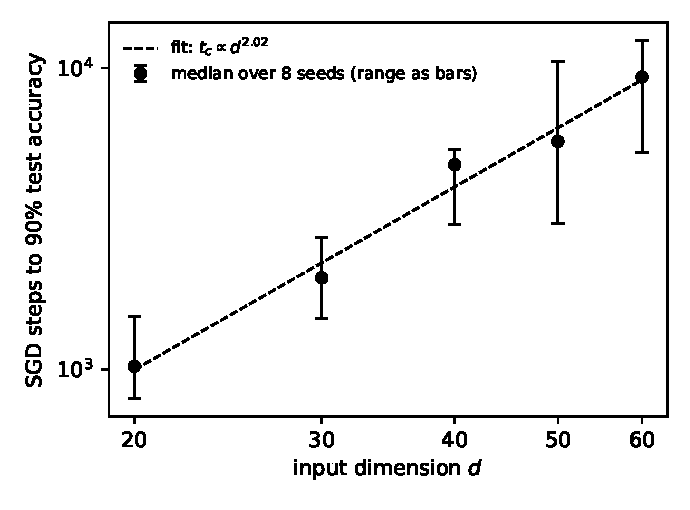
\includegraphics[width=0.62\linewidth]{../figures/parity-scaling.pdf}
\caption{Median SGD steps to \ParityThresh{} test accuracy against input dimension for a
hidden 3-sparse parity, log-log, \ParitySeeds{} seeds per point, bars spanning
the seed range. The fitted exponent \ParitySlope{} is the measured price of the
search in the recipe stated in the text.}
\label{fig:parity}
\end{figure}

What the experiment does and does not show. It shows one recipe's cost growing
as the power law the class floor predicts, in the regime where the recipe's
steps are noisy correlational queries. It does not measure the floor itself,
since no experiment can quantify over algorithms, and it says nothing about
structural adversaries, for which noiseless parity is easy. It is the empirical
face of the no-aiming postulate for the class that trains, and nothing more.
